\documentclass[11pt]{article}
\usepackage[T1]{fontenc}
\usepackage{lmodern,amsmath,amssymb,graphicx,xcolor,booktabs,array,enumitem}
\usepackage[letterpaper,margin=0.78in]{geometry}
\usepackage[colorlinks=true,linkcolor=blue,urlcolor=teal]{hyperref}
\usepackage{fancyhdr}
\definecolor{ink}{HTML}{172C3B}
\definecolor{teal}{HTML}{087F82}
\definecolor{blue}{HTML}{265DAB}
\pagestyle{fancy}\fancyhf{}
\fancyhead[L]{\footnotesize OpenAI math: independent illustrated reading editions}
\fancyfoot[C]{\thepage}
\setlength{\headheight}{15pt}
\setlength{\parindent}{0pt}\setlength{\parskip}{7pt}
\setlength{\emergencystretch}{2em}
\hypersetup{pdfauthor={Independent explanatory edition prepared with OpenAI Codex}}
\begin{document}
\begin{center}{\LARGE\bfseries How long can a coloring hide a progression?}\par\vspace{12pt}{\large An illustrated reader for superexponential van der Waerden bounds}\par\vspace{16pt}Independent reading edition, October 14, 2026\end{center}
\section*{Start here}Color the positive integers with two colors. A run of equally spaced numbers is an arithmetic progression: $2,5,8$ has common difference three. A progression is monochromatic when all its entries have the same color, even if other colors occur between them. How long can an interval be colored before a monochromatic progression becomes unavoidable?

This is an avoidance problem, so a long successful coloring proves a \emph{lower} bound. It says that the unavoidable point lies farther away. It does not say that every coloring of that length succeeds. The quantifiers are the heart of the question.

The source claims a construction whose avoided length grows superexponentially in the required progression length. Its argument combines circular coordinates, arithmetic dilation, geometric squared norms, probability, and a digit construction. This guide builds the intuition with small examples before explaining how those ingredients connect. The tiny colorings are checks of definitions, not miniature versions of the full asymptotic proof.
\paragraph{Reading prerequisites.} Ordinary arithmetic is enough for the opening examples. Later chapters introduce the specialized vocabulary; checking every original proof requires additional study.\par\textbf{Attribution.} Original manuscript by OpenAI. Added explanations and figures prepared with OpenAI Codex. This is not an official revision or independent theorem validation.\par\href{https://github.com/openai/math/tree/1581d4cbdd69a0faf34b2089614fe2a814316a6a/preprints/Quantitative-Superexponential-Bounds-for-van-der-Waerden-Numbers-September-23-2026}{Pinned original manuscript and citation}.\newpage\section*{The source claim, precisely}The source's Theorem 1.1 states that one absolute threshold $K_0$ works for all $r\ge2$ and $k\ge K_0$:
\[W_r(k)>k^{ck\lfloor\log_2r\rfloor},\qquad c=10^{-5}.\]
Here $W_r(k)$ is the least interval length forcing a monochromatic $k$-term progression in every $r$-coloring. For fixed $r$, the source concludes $W_r(k)^{1/k}\to\infty$. The charted formula supplies no numerical value for $K_0$.\paragraph{How to read this edition.} Each chapter gives one concrete illustration, then explains how it connects to the source. Captions identify toys and original constructions. Source anchors use the original manuscript\textquotesingle s section and page numbering. The expanded PDF places this guide before the complete unchanged original PDF, preserving the original page numbers and bibliography.\subsection*{Your route through the argument}\begin{enumerate}\item Read the quantifiers through an eight-position example
\item A circle has no cut; a coordinate interval does
\item Squared norm turns a line into a quadratic
\item A dilation removes troublesome small periods
\item Many bad events can still have total probability below one
\item Why the conclusion is stronger than beating one exponential
\end{enumerate}\paragraph{Verification scope.} The accompanying code checks the displayed finite examples and preserves original-file hashes. These checks do not replace the analytic, algebraic, asymptotic, or formal proof obligations in the source.\newpage\section*{Read the quantifiers through an eight-position example}
\begin{center}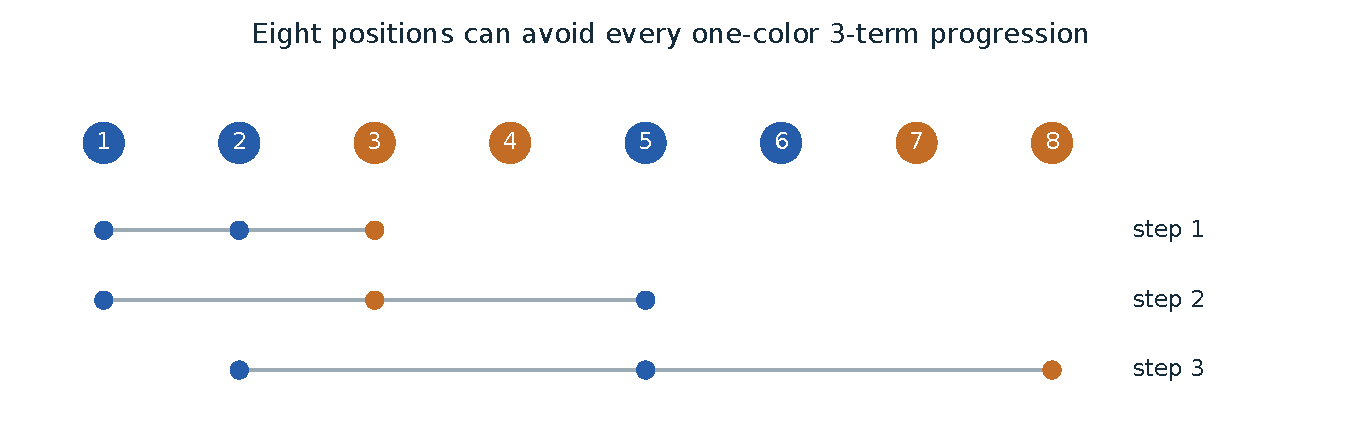
\includegraphics[width=\linewidth,height=2.35in,keepaspectratio]{figures/01-coloring.pdf}\end{center}
{\small\color{teal}\textbf{Figure 1.} An exhaustively checked coloring of eight positions avoids all monochromatic three-term progressions. The lower rows illustrate three possible spacings; all spacings are checked by the script.\par}
Start with the displayed eight-position coloring. A contiguous run is only one possible progression: step two and step three count too. To check the coloring, list every $a,a+d,a+2d$ with $d\ge1$ and $a+2d\le8$, then inspect the three colors. The script performs this complete check, rather than checking only the three rows drawn.

It also enumerates every binary coloring of nine positions and finds that none avoids every three-term progression. These two finite statements give $W_2(3)=9$: a witness at eight proves $W_2(3)>8$, while exhaustive failure at nine proves $W_2(3)\le9$.

\paragraph{Why this is not the large theorem.} The source addresses arbitrary sufficiently large $k$. A finite search can settle this tiny case but cannot establish an eventual growth law for every larger $k$. The source instead describes families of colorings and bounds all the ways a bad progression could occur.

\paragraph{Try it.} Does a red-blue-red alternating coloring avoid a monochromatic three-term progression? No: positions $1,3,5$ already share a color. Regular-looking colorings can create the very patterns we want to avoid.
{\footnotesize\color{blue}\textbf{Source anchor:} Section 1: definition of W\_r(k) and Theorem 1.1.\par}
\newpage\section*{A circle has no cut; a coordinate interval does}
\begin{center}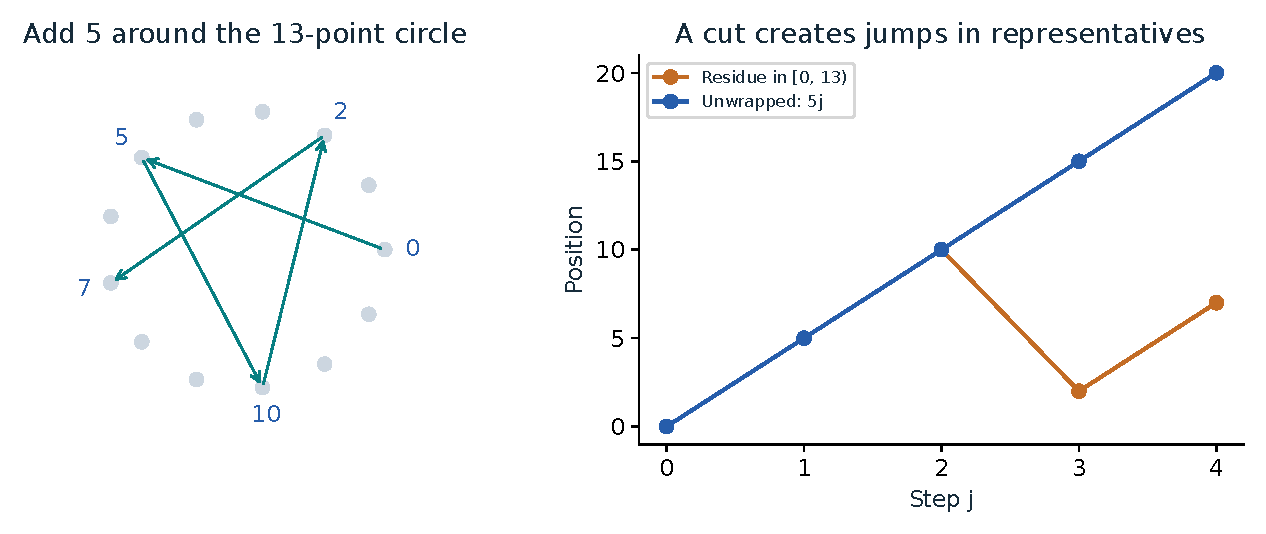
\includegraphics[width=\linewidth,height=2.35in,keepaspectratio]{figures/02-circle.pdf}\end{center}
{\small\color{teal}\textbf{Figure 2.} The residues 0, 5, 10, 2, 7 follow a constant step modulo 13. Representatives in an interval jump at the cut; their unwrapped values 0, 5, 10, 15, 20 remain affine.\par}
A cyclic group is a clock with a chosen number of positions. Adding five on a thirteen-position clock moves by the same amount every time. Yet the written representatives jump from ten to two because the display resets after twelve. Confusing the representatives with the underlying circular motion loses information.

The source uses a much larger cyclic group of order $q^D$. Its coordinate maps are $x_i(n)=n/q^i\pmod1$ and a second family $y_i(n)=\lambda x_i(n)$. A coordinate mesh records which short interval contains each coordinate. In the second family the intervals become finer near the cut, where an apparently short circular step can become a large change of real representative.

The proof needs a controlled alternative: a progression has enough of both outer colors, or its centered representatives follow a globally affine line. The little clock illustrates the obstacle, not a proof of that alternative. Getting a consistent lift in all coordinates is an obligation discharged by the paper's mesh and short-period arguments.

\paragraph{Vocabulary.} Affine means ``starting point plus step times index'': $u+jv$. A lift chooses real representatives for circular coordinates in a consistent way.
{\footnotesize\color{blue}\textbf{Source anchor:} Sections 2 and 5: cyclic coordinates, adaptive mesh, balanced-or-affine alternative.\par}
\newpage\section*{Squared norm turns a line into a quadratic}
\begin{center}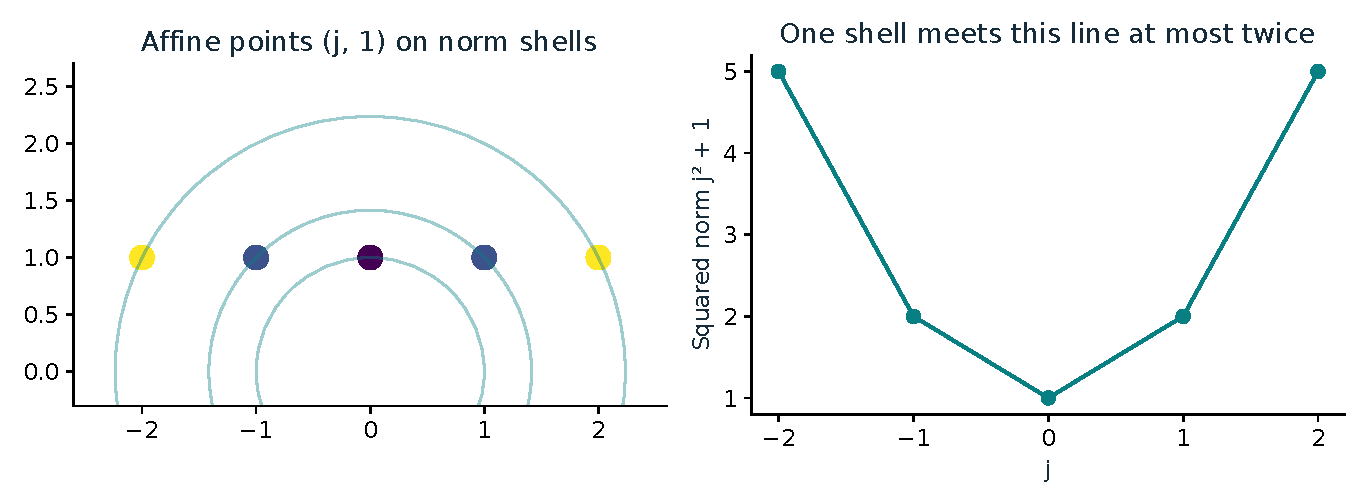
\includegraphics[width=\linewidth,height=2.35in,keepaspectratio]{figures/03-norm.pdf}\end{center}
{\small\color{teal}\textbf{Figure 3.} For the toy affine points (j,1), the squared norm is j$^2$+1. A circle of a fixed radius meets this line at at most two points.\par}
For a vector $(x,y)$, its squared Euclidean norm is $x^2+y^2$. On the horizontal line $(j,1)$ it becomes $j^2+1$, which is quadratic rather than linear. The five points in the diagram therefore have squared norms $5,2,1,2,5$. Equal norm values occur symmetrically on the two sides of the nearest point to the origin.

More generally,
\[\|u+jv\|^2=\|u\|^2+2j\langle u,v\rangle+j^2\|v\|^2.\]
The coefficients are fixed once the line is fixed. This limited structure helps count possible norm patterns along a progression.

The actual construction attaches a random flip to a key made from a coordinate box and an integer squared-norm band. Repeated occurrences of the same key reuse the same random bit. They are not fresh independent coin tosses. The source proves that each key occurs at most four times along the relevant progression and controls how many distinct key words need consideration.

Our exact-circle picture has at most two intersections. It does not replace the source's four-occurrence result for boxes and rounded bands. Its role is to show why squared norms supply usable structure.
{\footnotesize\color{blue}\textbf{Source anchor:} Section 6: norm-indexed perturbation; Section 1 construction overview.\par}
\newpage\section*{A dilation removes troublesome small periods}
\begin{center}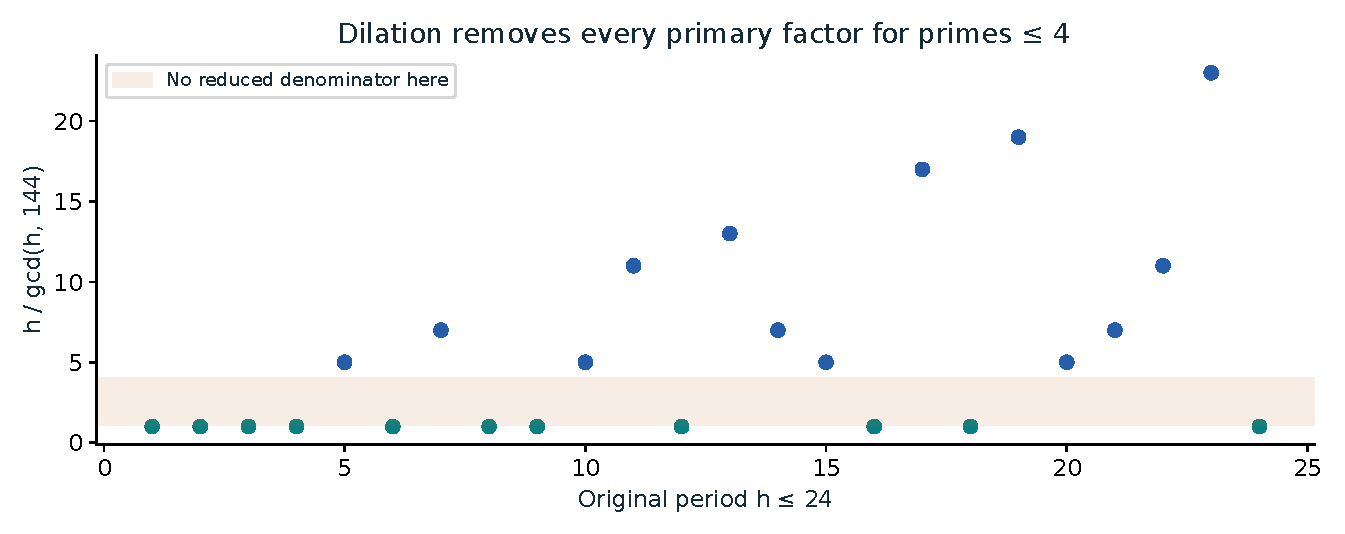
\includegraphics[width=\linewidth,height=2.35in,keepaspectratio]{figures/04-periods.pdf}\end{center}
{\small\color{teal}\textbf{Figure 4.} In this arithmetic example, $\lambda$=144 contains the full powers of 2 and 3 needed for every h$\le$24. The reduced denominator h/gcd(h,144) is either 1 or greater than 4.\par}
Think of a rational circular step $t/h$. Multiplying by $\lambda$ changes it to $\lambda t/h$, whose reduced denominator is
\[s=\frac{h}{\gcd(h,\lambda t)}.\]
If $\lambda$ contains all the relevant prime-power factors of $h$, that denominator collapses to one: the rational motion vanishes on the circle. Otherwise its remaining prime factors can be forced to be large.

For the plot, take $h\le24$, cutoff four, $t=1$, and $\lambda=2^4 3^2=144$. A denominator of twelve collapses to one; ten leaves five; twenty-one leaves seven. There are no remaining denominators two, three, or four. Every plotted value is computed with integer gcd arithmetic.

The source makes the analogous choice with a growing dimension $D$, cutoff $D^2$, and all potential periods up to $2\lceil k^{1/2}\rceil$. Lemma 2.1 proves that the residual period is one or exceeds $D^2$. This creates a clean separation of scales for the later geometric tests.

The sample parameters explain the arithmetic mechanism only. They are not a valid instance of all the source's simultaneous large-$k$ parameter requirements.
{\footnotesize\color{blue}\textbf{Source anchor:} Lemma 2.1 and equations (2.1)-(2.3).\par}
\newpage\section*{Many bad events can still have total probability below one}
\begin{center}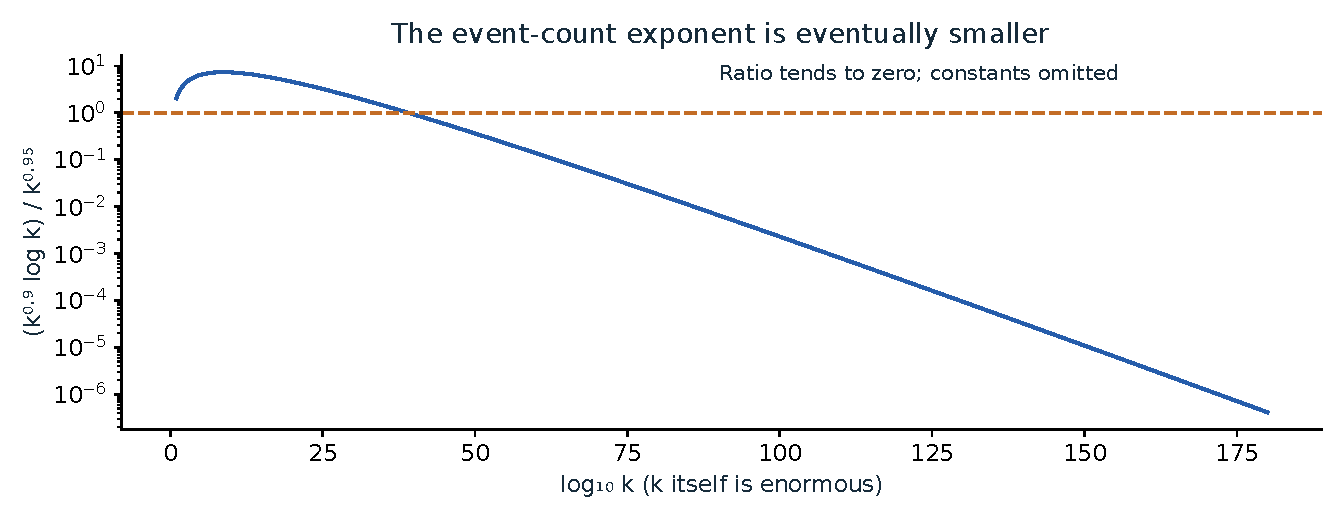
\includegraphics[width=\linewidth,height=2.35in,keepaspectratio]{figures/05-probability.pdf}\end{center}
{\small\color{teal}\textbf{Figure 5.} The plotted ratio (k\textasciicircum{}0.9 log k)/k\textasciicircum{}0.95 tends to zero. It compares exponent scales from the proof overview, omitting constants; it is not a computed probability of success.\par}
Suppose there are $N$ bad events, each with probability at most $e^{-B}$. Even if the events overlap, the union bound gives probability at most $Ne^{-B}$ that any occurs. Writing $N=e^A$ reveals the useful comparison: $e^{A-B}<1$ when $A<B$. Independence is not needed for that final union bound, although it matters when estimating each event.

The source organizes progressions by their label and key words so that identical words do not get counted repeatedly as different constraints. Its overview gives a logarithmic count $O(k^{9/10}\log k)$, compared with the rare-flip scale $pk=k^{19/20}$ for $p=k^{-1/20}$. Their ratio tends to zero because $\log k$ grows more slowly than $k^{1/20}$.

This convergence is slow. The horizontal axis is already $\log_{10}k$, not $k$. A plot of the bare expressions is not a usable threshold for the source theorem: hidden constants and all other parameter conditions must hold too.

The proof also uses local tests and a finite local lemma in constructing its outer coloring. This schematic union-bound calculation explains the final scale comparison without asserting that the entire construction is one independent random coloring.
{\footnotesize\color{blue}\textbf{Source anchor:} Sections 3-6; overview on original page 3.\par}
\newpage\section*{Why the conclusion is stronger than beating one exponential}
\begin{center}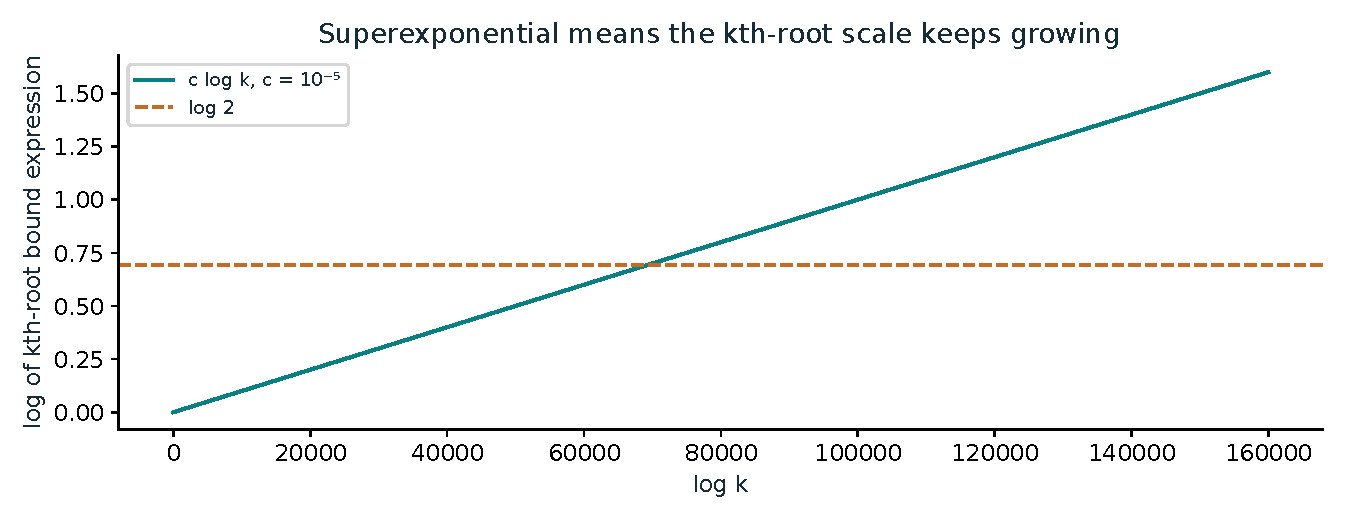
\includegraphics[width=\linewidth,height=2.35in,keepaspectratio]{figures/06-growth.pdf}\end{center}
{\small\color{teal}\textbf{Figure 6.} The two-color lower-bound expression has logarithmic kth-root scale c log k. The constant line log 2 represents the kth root of 2\textasciicircum{}k. The source theorem applies only beyond its unspecified threshold.\par}
An exponential $A^k$ has constant $k$th root $A$. By contrast, $(k^{ck})^{1/k}=k^c$ grows without bound whenever $c>0$. Taking one more logarithm gives the straight line $c\log k$ in the figure. Even a tiny fixed positive $c$ eventually exceeds every constant exponential base on this scale.

This does not mean the bound is numerically impressive at everyday values of $k$. Here $c=10^{-5}$, and the theorem has an unspecified sufficiently-large threshold. The distinction between eventual growth and useful finite sizes is essential.

To pass from two colors to arbitrary $r$, the source uses a deterministic digit product. Combining $\lfloor\log_2r\rfloor$ binary color choices uses at most $r$ colors, which explains why that integer appears in the exponent. The transfer also has to control cyclic progressions and carries; simply writing binary labels is not the whole proof.

\paragraph{Check your understanding.} A successful coloring proves a lower bound on the unavoidable length. A theorem forcing a progression in every coloring proves an upper bound. Reversing those statements reverses the meaning of the result.
{\footnotesize\color{blue}\textbf{Source anchor:} Theorem 1.1 and Section 7: transfer to intervals and additional colors.\par}
\newpage\section*{A vocabulary you can return to}
\paragraph{Arithmetic progression}Equally spaced terms with a positive common difference.
\paragraph{Monochromatic}All selected terms have the same color.
\paragraph{Cyclic group}Addition with wraparound modulo an integer.
\paragraph{Affine lift}Consistent real representatives of the form u+jv.
\paragraph{Union bound}The probability of any bad event is at most the sum of their probabilities.
\paragraph{Superexponential here}For fixed color count, the kth root of W\_r(k) tends to infinity.
\section*{What this edition checks}The guide checks the finite coloring search, the displayed period reductions, and the arithmetic behind the plots. It does not audit every mesh estimate, local-lemma dependency, word count, or cyclic-to-integer transfer. The original proof and bibliography follow unchanged in the expanded edition. Later coefficient refinements in separate repositories have their own assumptions and are not substituted for the source theorem here.
\paragraph{A useful self-test.} Explain what each plotted quantity counts, which examples are illustrative, and where the source needs a statement for every input or every sufficiently large size. If a picture seems to establish the full theorem by itself, revisit its caption and source anchor.\paragraph{Sources and reuse.}\href{https://github.com/openai/math/tree/1581d4cbdd69a0faf34b2089614fe2a814316a6a/preprints/Quantitative-Superexponential-Bounds-for-van-der-Waerden-Numbers-September-23-2026}{Quantitative Superexponential Bounds for van der Waerden Numbers}, OpenAI. Original bibliography and manuscript-specific citation are included with the source. Source snapshot: \texttt{1581d4cbdd69}. This derivative is distributed under Apache-2.0 with the original attribution; see the repository LICENSE and NOTICE.\end{document}